%%%%%%%%%%%%%%%%%%%%%%%%%%%%%%%%%%%%%%%%%
% Dreuw & Deselaer's Poster
% LaTeX Template
% Version 1.0 (11/04/13)
%
% Created by:
% Philippe Dreuw and Thomas Deselaers
% http://www-i6.informatik.rwth-aachen.de/~dreuw/latexbeamerposter.php
%
% This template has been downloaded from:
% http://www.LaTeXTemplates.com
%
% License:
% CC BY-NC-SA 3.0 (http://creativecommons.org/licenses/by-nc-sa/3.0/)
%
%%%%%%%%%%%%%%%%%%%%%%%%%%%%%%%%%%%%%%%%%

%----------------------------------------------------------fselec------------------------------
%	PACKAGES AND OTHER DOCUMENT CONFIGURATIONS
%----------------------------------------------------------------------------------------

\documentclass[final,hyperref={pdfpagelabels=false, brazil}]{beamer}

\usepackage[T1]{fontenc}
\usepackage[utf8]{inputenc}

\usepackage[orientation=portrait,size=a0,scale=1.4]{beamerposter} % Use the beamerposter package for laying out the poster with a portrait orientation and an a0 paper size

\usetheme{I6pd2} % Use the I6pd2 theme supplied with this template

\usepackage[english]{babel} % English language/hyphenation

\usepackage{amsmath,amsthm,amssymb,latexsym} % For including math equations, theorems, symbols, etc

%\usepackage{times}\usefonttheme{professionalfonts}  % Uncomment to use Times as the main font
%\usefonttheme[onlymath]{serif} % Uncomment to use a Serif font within math environments

\boldmath % Use bold for everything within the math environment

\usepackage{booktabs} % Top and bottom rules for tables

\graphicspath{{figures/}} % Location of the graphics files

\usecaptiontemplate{\small\structure{\insertcaptionname~\insertcaptionnumber: }\insertcaption} % A fix for figure numbering



%----------------------------------------------------------------------------------------
%	TITLE SECTION 
%----------------------------------------------------------------------------------------

\title{\huge Segmenta\c c\~ao e classifica\c c\~ao de Big Data} % Poster title

\author{Gustavo Kendi Tsuji} % Author(s)

\institute{Universidade de São Paulo} % Institution(s)

%----------------------------------------------------------------------------------------
%	FOOTER TEXT
%----------------------------------------------------------------------------------------

\newcommand{\leftfoot}{http://www.LaTeXTemplates.com} % Left footer text

\newcommand{\rightfoot}{gustavokt@gmail.com} % Right footer text

%----------------------------------------------------------------------------------------

\begin{document}

\addtobeamertemplate{block end}{}{\vspace*{2ex}} % White space under blocks

\begin{frame}[t] % The whole poster is enclosed in one beamer frame

\begin{columns}[t] % The whole poster consists of two major columns, each of which can be subdivided further with another \begin{columns} block - the [t] argument aligns each column's content to the top

\begin{column}{.02\textwidth}\end{column} % Empty spacer column

\begin{column}{.465\textwidth} % The first column

%----------------------------------------------------------------------------------------
%	INTRODUCTION
%----------------------------------------------------------------------------------------
            
\begin{block}{Introdu\c c\~ao}

\begin{itemize}

\item Na \emph{internet}, é possível encontrar mais de 60 trilhões de páginas indexadas pelo Google\cite{GOO01}. Só o Facebook possui \emph{data warehouses} com mais de 300 \emph{petabytes} e um tráfego de mais de 600 \emph{terabytes} diários\cite{FAC01}. Se o armazenamento desse volume de dados já era complexo, hoje, o desafio é extrair conhecimento dessas informações. Trata-se de um ativo intangível importante abre a possibilidade do desenvolvimento de novos produtos ou serviços bem como um melhor entendimento sobre comportamento dos clientes e funcionamento de processos, otimização da produção e outras melhorias.

\item É desta questão que nasce o \emph{Big Data}. A interpretação e extração de informações possibilitam uma melhor compreensão de vários aspectos, tanto nas esferas micro e macro na empresa. A utilização de \emph{Big Data} a favor da companhia pode conferir uma grande vantagem competitiva, bem como uma diferenciação, sendo considerado um ativo estratégico muito valioso.

\end{itemize}

\end{block}


%----------------------------------------------------------------------------------------
%	OBJECTIVES
%----------------------------------------------------------------------------------------

\begin{block}{Objetivos}

\begin{enumerate}
\item Realizar uma segmentação e analisar os clusters 
\item Classificar os dados usando 2 algoritmos a partir da clusterização realizada anteriormente e verificar a assertividade, analisando aspectos positivos e negativos de cada um
\end{enumerate}


\end{block}


%----------------------------------------------------------------------------------------
%	MATERIALS
%----------------------------------------------------------------------------------------

%\begin{block}{Materials}

%\begin{columns} % Subdivide the first main column
%\begin{column}{.54\textwidth} % The first subdivided column within the first main column
%\begin{itemize}
%\item Vestibulum nisl, quis euismod velit eros in ligula.
%\begin{itemize}
%\item Cras rhoncus quam et augue convallis in elementum urna tincidunt.
%\end{itemize}
%\item Proin ut vestibulum augue.
%\begin{itemize}
%\item Donec dapibus sagittis neque eu ultrices.
%\end{itemize}
%\end{itemize}
%\end{column}

%\begin{column}{.43\textwidth} % The second subdivided column within the first main column
%\centering
%\begin{figure}
%
\includegraphics[width=0.8\linewidth]{placeholder.jpg}
%\caption{Figure caption}
%\end{figure}
%\end{column}
%\end{columns} % End of the subdivision

%\begin{itemize}
%\item Curabitur sapien ligula, faucibus in feugiat quis, vestibulum a turpis.
%\begin{itemize}
%\item Phasellus quis nunc neque. Suspendisse mauris diam, suscipit non gravida in, placerat id enim. Ut nec ipsum in lectus ultrices sagittis.
%\item Ut nec ipsum in lectus ultrices sagittis.
%\item Phasellus quis nunc neque.
%\end{itemize}
%\end{itemize}

%\end{block}

%----------------------------------------------------------------------------------------
%	METHODS
%----------------------------------------------------------------------------------------

\begin{block}{Metodologia}


\begin{itemize}
\item Realização de experimento quantitativo  segmentação e classificação de dados. O estudo será realizado utilizando uma base de dados disponível em www.kaggle.com. com mais de 800 mil registros com informações relacionados como perfil do mutuário, detalhes das transações, entre outros. Esta base pertence a Loan Club, uma empresa de empréstimos com um sistema online.

\item A análise consiste em:
\begin{itemize}
\item Estudo dos algoritmos de Machine Learning (K Médias, Regressão Logística e Random Forest)
\item Análise descritiva dos clusters gerados
\item Criação de função de classificação da regressão logística
\item Visualização de uma árvore de classificação
\item Comparação da classificação da Regressão Logística e da Random Forest
\end{itemize}
\end{itemize}

\end{block}

%----------------------------------------------------------------------------------------
%	MATHEMATICAL SECTION
%----------------------------------------------------------------------------------------

\begin{block}{Fundamenta\c c\~ao te\'orica}

\begin{itemize}
\item Clusterização
\begin{itemize}
\item O K Médias é um método que, para uma dada quantidade k de clusters, tem como o objetivo de definir k centróides, um para cada cluster, tal que o conjunto de dados possa ser repartido de forma eficiente \cite{MacQueen}. Para um conjunto de observações \begin{math}(x_{1}, x_{2}, ..., x_{n})\end{math}, o objetivo é minimizar usando o princípio dos mínimos quadrados a função objetiva:
\begin{equation}
\label{eq:media}
\underset{S}{\arg\min} \sum_{i=1}^{k} \sum_{x \in S_{i}}\left \| x - \mu_{i} \right \|^{2}
\end{equation}
onde \begin{math}\mu_{i}\end{math} é o centróide da partição \begin{math}S_{i}\end{math}

\end{itemize}
\item Classificação
\begin{itemize}
\item A regressão logística é uma representação em fórmulas que tentam descrever ou simular eventos e sistemas reais com o propósito de prever comportamentos \cite{HASTIE}. Pode ser representada como
\begin{equation}
  \label{eq:regressao_linear}
  \begin{aligned}
Y &= \hat{\beta_{0}} + \sum_{j=1}^{p} (X_{j}\hat{\beta_{j}}), 
  \end{aligned}  
\end{equation}
onde \begin{math}Y\end{math} representa uma variável dependente contínua, \begin{math}X_{j}\end{math} as variáveis independentes 
Além disso, leva-se em consideração a probabilidade de que os eventos estudados ocorram. Para a predição das variáveis, é utilizado a função logit

\begin{equation}
  \label{eq:t}
  \begin{aligned}
    logit^{-1}(\alpha) &= \frac{1}{1+e^{-\alpha}} &= \frac{e^{\alpha}}{1+e^{\alpha}}
  \end{aligned}
\end{equation}

que estima os \emph{odds} como uma variável contínua. 

\end{itemize}

\begin{itemize}
\item A árvore de decisão é uma estrutura de modelo preditivo utilizado na aprendizagem supervisionada não parametrizada \cite{HASTIE}. Cada árvore possui um fluxo que define a classe a qual o dado pertence. É a base da random forest, que gera várias árvores para efetuar a classificação, já que apenas uma árvore poderia enviesar a classificação. Executando o algoritmo, um dado é classificado por diversas árvores e um resultado médio é o que define sua classificação.

\end{itemize}

\end{itemize}

\end{block}

%----------------------------------------------------------------------------------------

\end{column} % End of the first column

\begin{column}{.03\textwidth}\end{column} % Empty spacer column
 
\begin{column}{.465\textwidth} % The second column

%----------------------------------------------------------------------------------------
%	RESULTS
%----------------------------------------------------------------------------------------
%\begin{table}
%\begin{tabular}{l l l}
%\toprule
%\textbf{Treatments} & \textbf{Response 1} & \textbf{Response 2}\\
%\midrule
%Treatment 1 & 0.0003262 & 0.562 \\
%Treatment 2 & 0.0015681 & 0.910 \\
%Treatment 3 & 0.0009271 & 0.296 \\
%\bottomrule
%\end{tabular}
%\caption{Table caption}
%\end{table}

%\begin{itemize}
%\item Sollicitudin Vel Orci
%\item Maecenas Ultricies Feugiat Velit Non Mattis.
%\end{itemize}

%\begin{table}
%\begin{tabular}{l l l}
%\toprule
%\textbf{Treatments} & \textbf{Response 1} & \textbf{Response 2}\\
%\midrule
%Treatment 1 & 0.0003262 & 0.562 \\
%Treatment 2 & 0.0015681 & 0.910 \\
%Treatment 3 & 0.0009271 & 0.296 \\
%\bottomrule
%\end{tabular}
%\caption{Table caption}
%\end{table}
     
%\end{block}

%------------------------------------------------

\begin{block}{Resultados}

\begin{itemize}
\item Foram realizados clusterizações com 2 a 6 centróides e o resultado com o maior silhoute score foi com 2 clusters
\end{itemize}

\begin{figure}
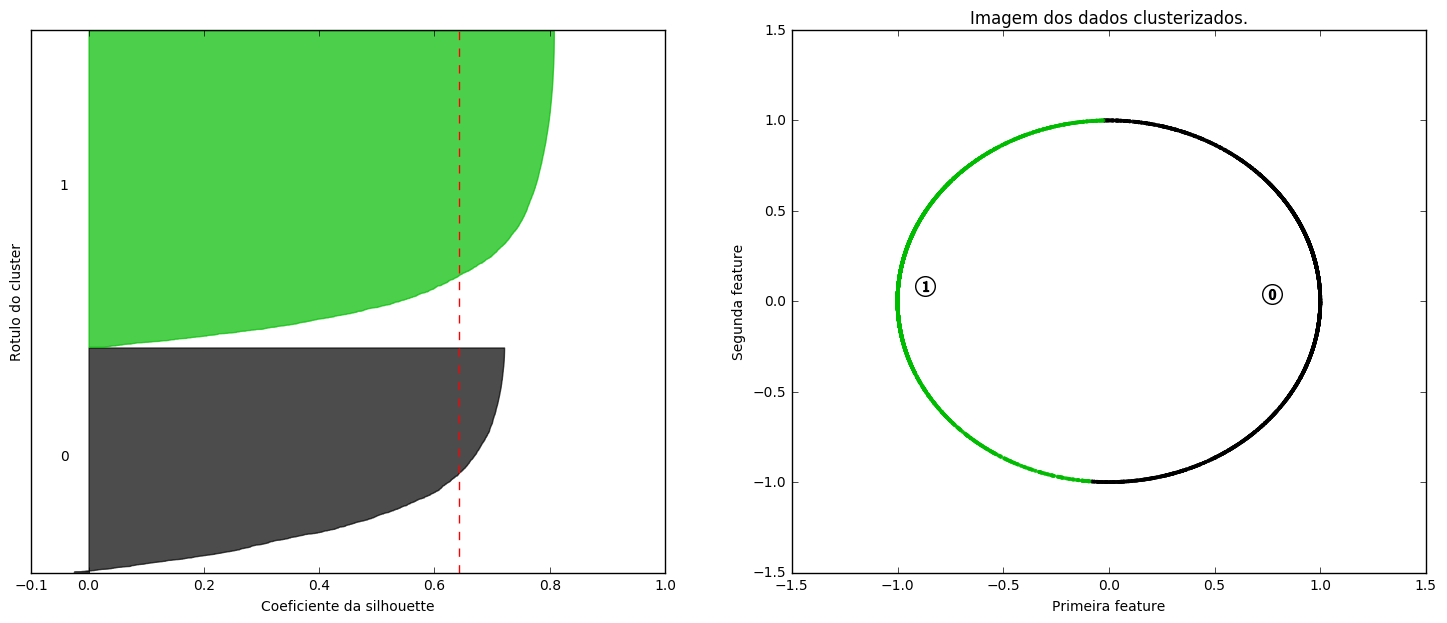
\includegraphics[width=0.85\linewidth]{silhoute2.png}
\caption{Clusterização}
\end{figure}

\begin{itemize}
\item Baseado na clusterização realizada pelo K médias, treinamos a base com a regressão logística e o random forest

\item Esta é uma das árvores geradas durante a execução do Random Forest

\begin{figure}
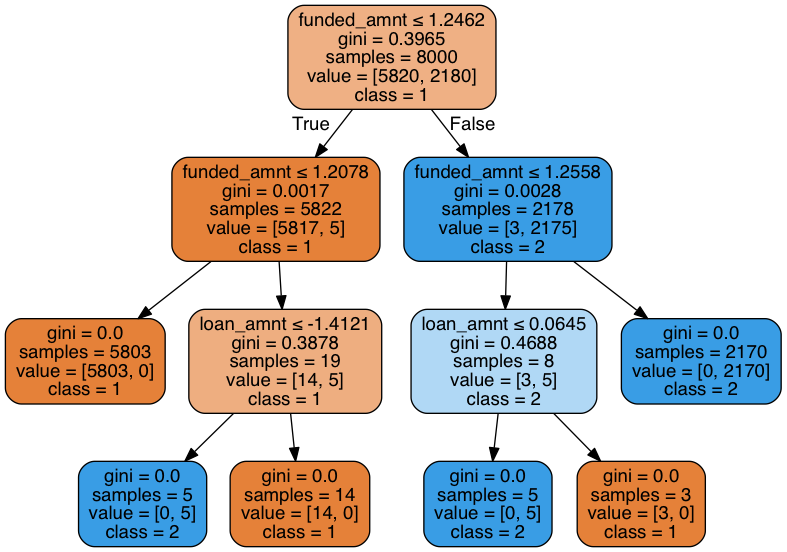
\includegraphics[width=0.7\linewidth]{loan.png}
\caption{Árvore de decisão para a base da Loan Club}
\end{figure}
\end{itemize}

\begin{itemize}
\item A
\begin{tabular}{ r r r r }

         & 1 & 2 & 3 \\
    1    & 29585 & 334   & 1307  \\
    2    & 715   & 58836 & 3957  \\
    3    & 1342  & 5006  & 164590
\end{tabular}

\begin{tabular}{ r r r r r }

  Classe & Precisão & Recall  & Falso Positivo & F-measure  \\
    1    & 0,93499  & 0,94744 & 0,00877        & 0,94117    \\
    2    & 0,91679  & 0,92643 & 0,02641        & 0,95234    \\
    3    & 0,96900  & 0,96286 & 0,05556        & 0,95241
\end{tabular}
\end{itemize}

\begin{itemize}

\item B
\begin{tabular}{ r r r r }

         & 1 & 2 & 3 \\
    1    & 27234 & 1470   & 524  \\
    2    & 2255   & 53129 & 5938  \\
    3    & 2153  & 9577   & 163392
\end{tabular}


\begin{tabular}{ r r r r r }

  Classe & Precisão & Recall  & Falso Positivo & F-measure  \\
    1    & 0,86069  & 0,93177 & 0,01864        & 0,89482    \\
    2    & 0,82786  & 0,86639 & 0,05405        & 0,84669    \\
    3    & 0,96195  & 0,93301 & 0,07136        & 0,94726
\end{tabular}
\end{itemize}

\begin{itemize}
\item Podemos observar que...

\end{itemize}

\end{block}

%----------------------------------------------------------------------------------------
%	CONCLUSION
%----------------------------------------------------------------------------------------

\begin{block}{Conclus\~ao}

\begin{itemize}
\item Opet volutpat ligula. Duis semper lorem eget dui dignissim porttitor. Nulla facilisi. In ullamcorper lorem quis dolor iaculis nec egestas enim ultricies. Cras ut mauris elit, ut lacinia dui. Proin in ante et libero hendrerit iaculis.




\end{itemize}

\end{block}

%----------------------------------------------------------------------------------------
%	REFERENCES
%----------------------------------------------------------------------------------------

\begin{block}{Refer\^encia Bibliogr\'afica}
        
\nocite{*} % Insert publications even if they are not cited in the poster
\small{\bibliographystyle{acm}
\bibliography{sample}}

\end{block}



%----------------------------------------------------------------------------------------
%	CONTACT INFORMATION
%----------------------------------------------------------------------------------------

%\setbeamercolor{block title}{fg=black,bg=orange!70} % Change the block title color

%\begin{block}{Contact Information}

%\begin{itemize}
%\item Web: \href{http://www.university.edu/smithlab}{http://www.university.edu/smithlab}
%\item Email: \href{mailto:john@smith.com}{john@smith.com}
%\item Phone: +1 (000) 111 1111
%\end{itemize}

%\end{block}

%----------------------------------------------------------------------------------------

\end{column} % End of the second column

\begin{column}{.015\textwidth}\end{column} % Empty spacer column

\end{columns} % End of all the columns in the poster

\end{frame} % End of the enclosing frame

\end{document}